%%%%%%%%%%%%%%%%%%%%%%%%%%%%%%%%%%%%%%%%%
% Formal Text-Rich Title Page 
% LaTeX Template
% Version 1.0 (27/12/12)
%
% This template has been downloaded from:
% http://www.LaTeXTemplates.com
%
% Original author:
% Peter Wilson (herries.press@earthlink.net)
%
% License:
% CC BY-NC-SA 3.0 (http://creativecommons.org/licenses/by-nc-sa/3.0/)
% 
% Instructions for using this template:
% This title page compiles as is. If you wish to include this title page in 
% another document, you will need to copy everything before 
% \begin{document} into the preamble of your document. The title page is
% then included using \titleGP within your document.
%
%%%%%%%%%%%%%%%%%%%%%%%%%%%%%%%%%%%%%%%%%

%----------------------------------------------------------------------------------------
%	PACKAGES AND OTHER DOCUMENT CONFIGURATIONS
%----------------------------------------------------------------------------------------

\documentclass{book}
\usepackage[utf8]{inputenc}
\usepackage{graphicx}
\usepackage{wrapfig}
\usepackage{caption}
\usepackage{subcaption}



\newcommand*{\plogo}{\fbox{$\mathcal{PL}$}} % Generic publisher logo

%----------------------------------------------------------------------------------------
%	TITLE PAGE
%----------------------------------------------------------------------------------------

\newcommand*{\titleGP}{\begingroup % Create the command for including the title page in the document
\centering % Center all text
\vspace*{\baselineskip} % White space at the top of the page

\rule{\textwidth}{1.6pt}\vspace*{-\baselineskip}\vspace*{2pt} % Thick horizontal line
\rule{\textwidth}{0.4pt}\\[\baselineskip] % Thin horizontal line

{\LARGE Florence Routes}\\[0.2\baselineskip] % Title

\rule{\textwidth}{0.4pt}\vspace*{-\baselineskip}\vspace{3.2pt} % Thin horizontal line
\rule{\textwidth}{1.6pt}\\[\baselineskip] % Thick horizontal line

\scshape % Small caps
Progettazione e Produzione Multimediale
\par % Location and year

\vspace*{2\baselineskip} % Whitespace between location/year and editors

Edited by \\[\baselineskip]
{\Large Terreni Maurizio\par} % Editor list
{\itshape Università degli Studi di Firenze \\ Ingegneria Informatica\par} % Editor affiliation

\vfill % Whitespace between editor names and publisher logo

{\scshape Anno Accademico 2013/2014} \\[0.3\baselineskip] % Year published


\endgroup}

%----------------------------------------------------------------------------------------
%	BLANK DOCUMENT
%----------------------------------------------------------------------------------------

\begin{document} 

\pagestyle{empty} % Removes page numbers

\titleGP % This command includes the title page


\newpage

\tableofcontents

\chapter*{Prefazione}
 

Lo scopo è quello di realizzare un progetto che consiste in una semplice applicazione web Desktop/ mobile Responsive,capace di organizzare la giornata di un turista in visita a Firenze.\\
I linguaggi come Jquery Mobile e php hanno reso possibile la realizzazione dell'interfaccia grafica e la gestione dei Point Of interest da parte dell'utente.\
L'aggiunta delle piattaforme come Facebook e Foursquare cerca di rendere l'itinerario molto più personalizzato,andando a elencare una serie di luoghi selezionati automaticamente in relazione ai gusti personali e ai locali con rating maggiore al momento della ricerca,così da offrire al turista una più ampia selezione di luoghi da visitare.  


 
\chapter{Florence Routes}
\begin{wrapfigure}{r}{0.5\textwidth}
  \vspace{-20pt}
  \begin{center}
   
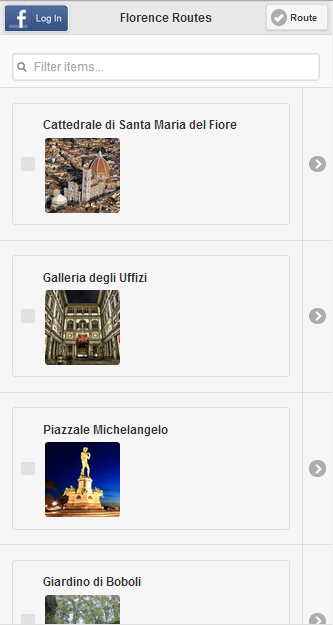
\includegraphics[width=0.40\textwidth]{img/fig1}
  \end{center}
  \vspace{-20pt}
  \caption*{Fig 1}
  \vspace{-10pt}
\end{wrapfigure}
\section{Selezione dei Point of interest}

Al primo avvio dell'applicazione (fig. 1) vengono elencati una serie di point of interest selezionabili attraverso un semplice click.\
Per conoscere le informazioni relative al POI desiderato basta premere il bottone (fig. 1.2)  al lato e si aprirà un popup (fig 1.3) contentente tutte le informazioni necessarie.\
Possiamo filtrare la ricerca dei luoghi attraverso (fig 1.4) il filtro ricerca inserendo il nome del monumento da ricerare e automaticcamte viene generata una lista contenete solo i POI che rispettano i criteri di ricerca.

\newpage
\begin{figure}
 \center
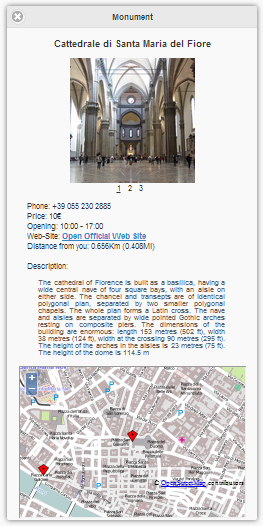
\includegraphics[width=.4\linewidth]{img/fig1-3}

  \caption{Fig 1.3}
  \label{fig:sub1}

\end{figure}
\begin{figure}
 \center
\begin{subfigure}{.5\textwidth}
  \centering
  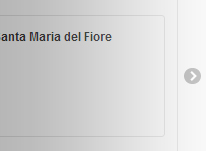
\includegraphics[width=.4\linewidth]{img/fig1-2}
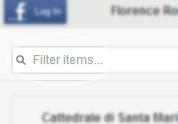
\includegraphics[width=.4\linewidth]{img/fig1-4}
  \caption{Fig 1.2}
  \label{fig:sub1}
\end{subfigure}
       \begin{subfigure}{.5\textwidth}
  \centering
  
  \caption{Fig 1.4}
  \label{fig:sub1}
\end{subfigure}
\end{figure}


\section{Routes}
\begin{wrapfigure}{r}{0.5\textwidth}
  \vspace{-20pt}
  \begin{center}
   
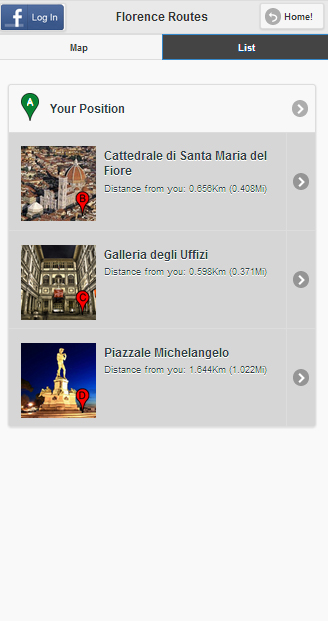
\includegraphics[width=0.30\textwidth]{img/fig1-6}
  \end{center}
  \vspace{-20pt}
  \caption*{Fig 1.6}
  \vspace{-10pt}
\end{wrapfigure}
L'utente, dopo aver selezionato almeno un monumento, è in grado di procedere con l'itinerario desiderato attraverso il click del pulsante Routes(fig. 1.5).
\ Automaticamente viene caricata la mappa di Firenze con indicato il tragitto più breve per raggiungere tutti i luoghi interessati, inoltre la mappa contiene delle label che consentono tramite un click di conoscere le informazioni del waypoint selezionato, in maniera da rendere l'itinerario più semplice e interattivo.\ \



Selezionando la colonna "Lista" (fig 1.6) viene elencato in ordine di itinerario la lista dei point of interest con le rispettive label della mappa (fig 1.7) e in aggiunta alcune informazioni:il nome del luogo,la distanza del monumento dall'utente.\

\begin{figure}
 \center
\begin{subfigure}{.5\textwidth}
  \centering
  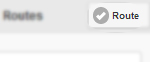
\includegraphics[width=.4\linewidth]{img/fig1-5}
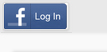
\includegraphics[width=.4\linewidth]{img/fig1-8}
  \caption{Fig 1.5}
  \label{fig:sub1}
\end{subfigure}
       \begin{subfigure}{.5\textwidth}
  \centering
  
  \caption{Fig 1.8}
  \label{fig:sub1}
\end{subfigure}
\end{figure}



\begin{figure}
 \center

  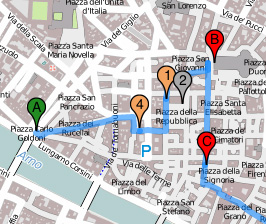
\includegraphics[width=.4\linewidth]{img/fig1-7}

  \caption*{Fig 1.7}

\end{figure}

\newpage
\section{Facebook e Foursquare}
\begin{wrapfigure}{r}{0.5\textwidth}
  \vspace{-20pt}
  \begin{center}
   
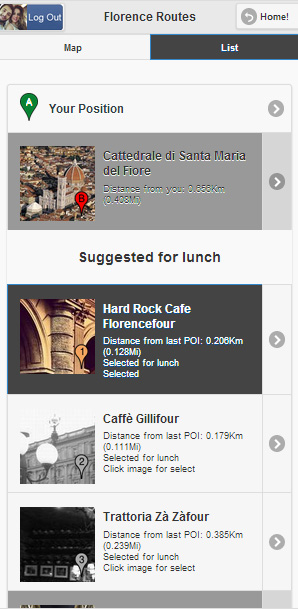
\includegraphics[width=0.40\textwidth]{img/fig1-9}
  \end{center}
  \vspace{-20pt}
  \caption*{Fig 1.9}
  \vspace{-10pt}
\end{wrapfigure}
Nella pagina principale è possibile effettuare il Login del proprio utente con Facebook (fig 1.8) dove una volta cliccato il link potremmo inserire le credenziali per accedere. Finito di autenticarsi, apparirà al posto dell'icona di facebook l'immagine del profilo e nel footer il nome utente in maniera da garantire che la connessione è stata stabilita con successo ed è possibile utilizzare l'applicazione con tutte le sue funzionalità.\

La selezione dei POI è indifferente se effettuata essendo connessi a facebook oppure no. 
L'utente ha la possibilità di collegarsi a facebook ed iniziare il suo itinerario.\
Nella mappa verranno aggiunte,automaticamente, alcune particolari label con i point of interest selezionati in basi ai like dell'account facebook.\

Nella colonna "Lista" (fig 1.10) appare l'elenco di tutti i luoghi selezionati,in aggiunta alcuni suggerimenti proposti in base ai propri gusti e al rating su Foursquare, seguiti da informazioni come la distanza del luogo dall'ultimo point of interest della lista.
L'utente è in grado di aggiungere o eliminare dalla mappa un luogo suggerito, semplicemente selezionandolo nella lista. \
Automaticamente la riga del luogo selezionato si evidenzierà in modo da rendere intuitivo quali luoghi si andranno a visitare.
Appena un utente seleziona o disattiva un luogo suggerito, la mappa viene aggiornata automaticamente ricalcolando l'itinerario.
I luoghi suggeriti sono suddivisi in tre fasce:
\begin{enumerate}
\item Pranzo
\item Pomerioggio
\item Sera
\end{enumerate}

La prima contiene un elenco dei possibili ristoranti dove un turista potrebbe fermarsi a pranzo.\
La seconda contiene un elenco di alcuni possibili luoghi calcolati dai gusti dell'utente,come per esempio alcuni negozi dove poter fare shopping.\
La terza contiene un elenco di locali dove poter rimanere sia a cena che dopo in maniera da garantire un completo intrattenimento.\
Non sempre vengono calcolate tutte e tre le fasce infatti in base all'orario in cui viene calcolato l'itinerario alcune possono essere escluse.


\chapter{Programmazione}
\section{Selezione Dei Point of interest}
Ogni point of interest presente nella lista appartiene ad una specifica classe.\
Quando l'utente effettua un click su di uno specifico item viene chiamata una funzione jquery,la quale crea una lista e ad ogni click viene aggiunto in sequenza l'id del'item selezionato, in modo da ottenere un elenco dei soli punti che l'utente vuole visitare.\
Il pulsante "Route" consente di poter capire quando un utente è soddisfatto dei luoghi selezionati e quindi poter procedere con il calcolo dell'itinerario.\
Il pulsante è abilitato solo al momento in cui viene selezionato almeno un item in modo da non caricare la mappa senza alcun point of interest nella lista.
Ogni luogo presente al caricamento della pagina principale è salvato nel database, il record oltre a contenere il nome e l'id del point of interest contiene anche i dati come le coordinate, la descrizione , ecc.

\section{Routes}

Quando un utente preme il bottone Route ( caso in cui non si è connessi a facebook) viene caricata la mappa con i soli monumenti che l'utente ha deciso di visitare, successivanente vengono generati dei waypoint e dei marker che servono per riempire la mappa con l'itinerario e le label dei luoghi.\
Ad ogni marker viene associato un evento che mostra alcuni dati, come l'immagine e il Nome del luogo.
Tramite la geolocalizzazione è possibile sapere la posizione precisa dell'utente in maniera da fissare il punto di partenza dell'itinerario.
Ad ogni Marker è stato associato un valore e un colore in modo da distinguerli tra loro. 
Colori diversi corrispondono a categorie diverse, che possono essere:
\begin{enumerate}
\item Colore Verde - indica la posizione dell'utente all'interno della mappa.
\item Colore Rosso - indica la posizione di tutti i point of interest selezionati dall'utente 
\item Colore Giallo - inidica la posizione di tutti i point of interest ricavati da foursquere e selezionati dall'utente (presenti solo se l'utente ha effettuato il login con Facebbok)
\item Colore Grigio -  inidica la posizione di tutti i point of interest ricavati da foursquere ma non selezionati dall'utente  (presenti solo se l'utente ha effettuato il login con Facebbok)
\end{enumerate} 
\section{Facebook e Foursquare}

Quando l'utente effettua il login con facebook vengono letti automaticamente i likes, questo è reso possibile grazie alla libreria "facebook.php" che contiene tutte le api per effettuare query sull'utente connesso.\
Un Like di facebook è semplicemente un array che contiene i dati della pagina come per esempio il nome, la categoria , ecc.. \ Tramite una funzione php viene estratto dal like di Fecebook solo la categoria di appartenenza andando a generare un nuovo array.
Per semplificare la gestione, le numerose categorie di facebook (all'incirca più di mille) sono state raggruppate in un array di soli 10 elementi in maniera da renderne più flessibile l'utilizzo (per esempio all'interno della categoria Film sono stati ragruppati le voci come attore , regista , ecc..) e inoltre rendere piu precisa la ricerca dei luoghi. \
Questo array va a generare un gruppo di categorie utilizzate all'interno dell'applicazione per selezionare le tipologie dei luoghi da ricercare in foursquare.
Ogni categoria di facebook riscontrata incrementa un contatore delle categorie da noi generato. Al termine avremo per ogni componente il numero totale di likes di facebook.
Una volta finito di leggere i likes del'utente vengono prelevati i luoghi da foursquare suddividendoli in tre fasce:


\begin{enumerate}
\item Pranzo - Se l' utente si trova a selezionare i poi in una fascia oraria che va dalle 7 di mattina alle 14 del pomeriggio, tramite una query a Foursquare, vengono presi i primi tre ristoranti nel raggio di 1km con rating maggiore ed aggiunti ad una lista di items dedicata.

\item Pomeriggio - Entra in funzione l'array precedentemente inizializzato e tramite foursquare vengono selezionati tre items appartenenti alle categorie presenti nell'array ( esempio se ad un utente gli piace sia lo shopping sia lo sport verrà ricercato un negozio che vende articoli sportivi ).
\item Sera - in base alle categorie dei locali che piacciono all'utente vengono selezionati quattro items comopreso alcuni ristoranti dove poter fermari a cena.
\end{enumerate}

 
Caricati tutti i luoghi suggeriti, vengono automaticamente selezionati gli items in testa alla lista e aggiunti all'itinerario con una label di colore giallo, mentre per  gli items non selezionati viene solamente aggiunta una label di colore grigio.
Ad ogni luogo quindi è associata una variabile booleana che indica se essere compreso nell'itinerario o no.
Tramite il click sull'item viene chiamata una funzione in php che graize all'id del luogo modifica la variabile booleana.
 




\end{document}